
\documentclass[letterpaper,hide notes,xcolor={table,svgnames},pdftex,10pt]{beamer}
\def\showexamples{t}


%\usepackage[svgnames]{xcolor}

%% Demo talk
%\documentclass[letterpaper,notes=show]{beamer}

\usecolortheme{crane}
\setbeamertemplate{navigation symbols}{}

\usetheme{MyPittsburgh}
%\usetheme{Frankfurt}

%\usepackage{tipa}

\usepackage{hyperref}
\usepackage{graphicx,xspace}
\usepackage[normalem]{ulem}
\usepackage{multicol}
\usepackage{amsmath,amssymb,amsthm,graphicx,xspace}
\newcommand\SF[1]{$\bigstar$\footnote{SF: #1}}

\usepackage[default]{sourcesanspro}
\usepackage[T1]{fontenc}

\newcounter{tmpnumSlide}
\newcounter{tmpnumNote}

% old question code
%\newcommand\question[1]{{$\bigstar$ \small \onlySlide{2}{#1}}}
% \newcommand\nquestion[1]{\ifdefined \presentationonly \textcircled{?} \fi \note{\par{\Large \textbf{?}} #1}}
% \newcommand\nanswer[1]{\note{\par{\Large \textbf{A}} #1}}


 \newcommand\mnote[1]{%
   \addtocounter{tmpnumSlide}{1}
   \ifdefined\showcues {~\tiny\fbox{\arabic{tmpnumSlide}}}\fi
   \note{\setlength{\parskip}{1ex}\addtocounter{tmpnumNote}{1}\textbf{\Large \arabic{tmpnumNote}:} {#1\par}}}

\newcommand\mmnote[1]{\note{\setlength{\parskip}{1ex}#1\par}}

%\newcommand\mnote[2][]{\ifdefined\handoutwithnotes {~\tiny\fbox{#1}}\fi
% \note{\setlength{\parskip}{1ex}\textbf{\Large #1:} #2\par}}

%\newcommand\mnote[2][]{{\tiny\fbox{#1}} \note{\setlength{\parskip}{1ex}\textbf{\Large #1:} #2\par}}

\newcommand\mquestion[2]{{~\color{red}\fbox{?}}\note{\setlength{\parskip}{1ex}\par{\Large \textbf{?}} #1} \note{\setlength{\parskip}{1ex}\par{\Large \textbf{A}} #2\par}\ifdefined \presentationonly \pause \fi}

\newcommand\blackboard[1]{%
\ifdefined   \showblackboard
  {#1}
  \else {\begin{center} \fbox{\colorbox{blue!30}{%
         \begin{minipage}{.95\linewidth}%
           \hspace{\stretch{1}} Some space intentionally left blank; done at the blackboard.%
         \end{minipage}}}\end{center}}%
         \fi%
}



%\newcommand\q{\tikz \node[thick,color=black,shape=circle]{?};}
%\newcommand\q{\ifdefined \presentationonly \textcircled{?} \fi}

\usepackage{listings}
\lstset{%
  keywordstyle=\bfseries,
  aboveskip=15pt,
  belowskip=15pt,
  captionpos=b,
  identifierstyle=\ttfamily,
  escapeinside={(*@}{@*)},
  stringstyle=\ttfamiliy,
  frame=lines,
  numbers=left, basicstyle=\scriptsize, numberstyle=\tiny, stepnumber=0, numbersep=2pt}

\usepackage{siunitx}
\newcommand\sius[1]{\num[group-separator = {,}]{#1}\si{\micro\second}}
\newcommand\sims[1]{\num[group-separator = {,}]{#1}\si{\milli\second}}
\newcommand\sins[1]{\num[group-separator = {,}]{#1}\si{\nano\second}}
\sisetup{group-separator = {,}, group-digits = true}

%% -------------------- tikz --------------------
\usepackage{tikz}
\usetikzlibrary{positioning}
\usetikzlibrary{arrows,backgrounds,automata,decorations.shapes,decorations.pathmorphing,decorations.markings,decorations.text}

\tikzstyle{place}=[circle,draw=blue!50,fill=blue!20,thick, inner sep=0pt,minimum size=6mm]
\tikzstyle{transition}=[rectangle,draw=black!50,fill=black!20,thick, inner sep=0pt,minimum size=4mm]

\tikzstyle{block}=[rectangle,draw=black, thick, inner sep=5pt]
\tikzstyle{bullet}=[circle,draw=black, fill=black, thin, inner sep=2pt]

\tikzstyle{pre}=[<-,shorten <=1pt,>=stealth',semithick]
\tikzstyle{post}=[->,shorten >=1pt,>=stealth',semithick]
\tikzstyle{bi}=[<->,shorten >=1pt,shorten <=1pt, >=stealth',semithick]

\tikzstyle{mut}=[-,>=stealth',semithick]

\tikzstyle{treereset}=[dashed,->, shorten >=1pt,>=stealth',thin]

\usepackage{ifmtarg}
\usepackage{xifthen}
\makeatletter
% new counter to now which frame it is within the sequence
\newcounter{multiframecounter}
% initialize buffer for previously used frame title
\gdef\lastframetitle{\textit{undefined}}
% new environment for a multi-frame
\newenvironment{multiframe}[1][]{%
\ifthenelse{\isempty{#1}}{%
% if no frame title was set via optional parameter,
% only increase sequence counter by 1
\addtocounter{multiframecounter}{1}%
}{%
% new frame title has been provided, thus
% reset sequence counter to 1 and buffer frame title for later use
\setcounter{multiframecounter}{1}%
\gdef\lastframetitle{#1}%
}%
% start conventional frame environment and
% automatically set frame title followed by sequence counter
\begin{frame}%
\frametitle{\lastframetitle~{\normalfont(\arabic{multiframecounter})}}%
}{%
\end{frame}%
}
\makeatother

\makeatletter
\newdimen\tu@tmpa%
\newdimen\ydiffl%
\newdimen\xdiffl%
\newcommand\ydiff[2]{%
    \coordinate (tmpnamea) at (#1);%
    \coordinate (tmpnameb) at (#2);%
    \pgfextracty{\tu@tmpa}{\pgfpointanchor{tmpnamea}{center}}%
    \pgfextracty{\ydiffl}{\pgfpointanchor{tmpnameb}{center}}%
    \advance\ydiffl by -\tu@tmpa%
}
\newcommand\xdiff[2]{%
    \coordinate (tmpnamea) at (#1);%
    \coordinate (tmpnameb) at (#2);%
    \pgfextractx{\tu@tmpa}{\pgfpointanchor{tmpnamea}{center}}%
    \pgfextractx{\xdiffl}{\pgfpointanchor{tmpnameb}{center}}%
    \advance\xdiffl by -\tu@tmpa%
}
\makeatother
\newcommand{\copyrightbox}[3][r]{%
\begin{tikzpicture}%
\node[inner sep=0pt,minimum size=2em](ciimage){#2};
\usefont{OT1}{phv}{n}{n}\fontsize{4}{4}\selectfont
\ydiff{ciimage.south}{ciimage.north}
\xdiff{ciimage.west}{ciimage.east}
\ifthenelse{\equal{#1}{r}}{%
\node[inner sep=0pt,right=1ex of ciimage.south east,anchor=north west,rotate=90]%
{\raggedleft\color{black!50}\parbox{\the\ydiffl}{\raggedright{}#3}};%
}{%
\ifthenelse{\equal{#1}{l}}{%
\node[inner sep=0pt,right=1ex of ciimage.south west,anchor=south west,rotate=90]%
{\raggedleft\color{black!50}\parbox{\the\ydiffl}{\raggedright{}#3}};%
}{%
\node[inner sep=0pt,below=1ex of ciimage.south west,anchor=north west]%
{\raggedleft\color{black!50}\parbox{\the\xdiffl}{\raggedright{}#3}};%
}
}
\end{tikzpicture}
}


%% --------------------

%\usepackage[excludeor]{everyhook}
%\PushPreHook{par}{\setbox0=\lastbox\llap{MUH}}\box0}

%\vspace*{\stretch{1}

%\setbox0=\lastbox \llap{\textbullet\enskip}\box0}

\setlength{\parskip}{\fill}

\newcommand\noskips{\setlength{\parskip}{1ex}}
\newcommand\doskips{\setlength{\parskip}{\fill}}

\newcommand\xx{\par\vspace*{\stretch{1}}\par}
\newcommand\xxs{\par\vspace*{2ex}\par}
\newcommand\tuple[1]{\langle #1 \rangle}
\newcommand\code[1]{{\sf \footnotesize #1}}
\newcommand\ex[1]{\uline{Example:} \ifdefined \presentationonly \pause \fi
  \ifdefined\showexamples#1\xspace\else{\uline{\hspace*{2cm}}}\fi}

\newcommand\ceil[1]{\lceil #1 \rceil}


\AtBeginSection[]
{
   \begin{frame}
       \frametitle{Outline}
       \tableofcontents[currentsection]
   \end{frame}
}



\pgfdeclarelayer{edgelayer}
\pgfdeclarelayer{nodelayer}
\pgfsetlayers{edgelayer,nodelayer,main}

\tikzstyle{none}=[inner sep=0pt]
\tikzstyle{rn}=[circle,fill=Red,draw=Black,line width=0.8 pt]
\tikzstyle{gn}=[circle,fill=Lime,draw=Black,line width=0.8 pt]
\tikzstyle{yn}=[circle,fill=Yellow,draw=Black,line width=0.8 pt]
\tikzstyle{empty}=[circle,fill=White,draw=Black]
\tikzstyle{bw} = [rectangle, draw, fill=blue!20, 
    text width=4em, text centered, rounded corners, minimum height=2em]
    
    \newcommand{\CcNote}[1]{% longname
	This work is licensed under the \textit{Creative Commons #1 3.0 License}.%
}
\newcommand{\CcImageBy}[1]{%
	\includegraphics[scale=#1]{creative_commons/cc_by_30.pdf}%
}
\newcommand{\CcImageSa}[1]{%
	\includegraphics[scale=#1]{creative_commons/cc_sa_30.pdf}%
}
\newcommand{\CcImageNc}[1]{%
	\includegraphics[scale=#1]{creative_commons/cc_nc_30.pdf}%
}
\newcommand{\CcGroupBySa}[2]{% zoom, gap
	\CcImageBy{#1}\hspace*{#2}\CcImageNc{#1}\hspace*{#2}\CcImageSa{#1}%
}
\newcommand{\CcLongnameByNcSa}{Attribution-NonCommercial-ShareAlike}

\newenvironment{changemargin}[1]{% 
  \begin{list}{}{% 
    \setlength{\topsep}{0pt}% 
    \setlength{\leftmargin}{#1}% 
    \setlength{\rightmargin}{1em}
    \setlength{\listparindent}{\parindent}% 
    \setlength{\itemindent}{\parindent}% 
    \setlength{\parsep}{\parskip}% 
  }% 
  \item[]}{\end{list}} 




\title{Lecture 8 ---  Modelling Diagrams}

\author{Jeff Zarnett \\ \small \texttt{jzarnett@uwaterloo.ca}}
\institute{Department of Electrical and Computer Engineering \\
  University of Waterloo}
\date{\today}


\begin{document}

\begin{frame}
  \titlepage

 \end{frame}


\begin{frame}
\frametitle{Good Design}

We have talked at some length about the tools for defining the database, but we really should spend significant time on good design. 

Knowing how hammers work is not enough; we also need to understand what good architectural plans look like.

The first thing we would like to watch out for is redundancy in the database and eliminate it wherever possible. 

In short, if there is redundant data then there is the potential for data to get out of date or be in some other inconsistent state. 

\end{frame}



\begin{frame}
\frametitle{Design with Diagrams}

When we have some data that we would like to represent we need to turn it into some database tables. 

Going directly from some ideas about what data we need to the tables is sometimes difficult and may produce undesirable results. 

Instead, we should devise a plan for how it should be implemented and for that we will create diagrams. 

Diagrams are done on paper or a whiteboard or similar and it is very easy to visualize, understand, and change the design at that stage.


\end{frame}



\begin{frame}
\frametitle{Entity-Relationship Diagrams}

Entity-relationship diagrams have the following symbols and their meanings:

\begin{itemize}
	\item \textbf{Divided Rectangles} represent an entity; an entity has a title (the top part) and a list of the attributes of that entity (the bottom part).
	\item \textbf{Diamonds} represent a relationship set.
	\item \textbf{Undivided Rectangles} represent the attributes of a relationship set. 
	\item \textbf{Lines} link entity sets to relationship sets.
	\item \textbf{Dashed Lines} linked the attributes of a relationship set to its relationship set.
	\item \textbf{Double lines} indicate total participation of an entity in a relationship set.
	\item \textbf{Double Diamonds} represent identifying relationship sets linked to weak entity sets.
\end{itemize}

Note also that in rectangles, attributes that are or form part of the primary key are underlined. 

\end{frame}



\begin{frame}
\frametitle{E-R Diagram Example}

\begin{center}
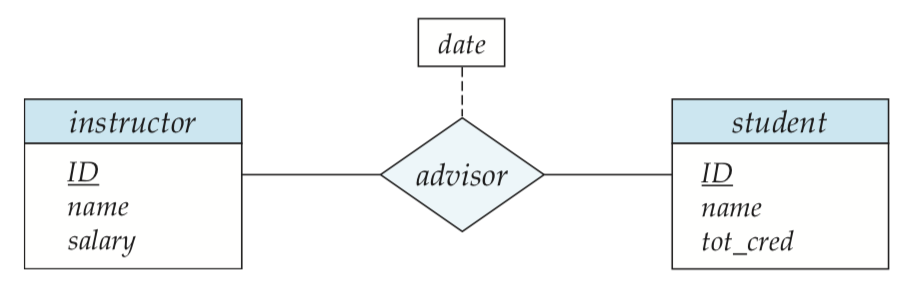
\includegraphics[width=0.9\textwidth]{images/er-with-attr}\\
\end{center}


\end{frame}



\begin{frame}
\frametitle{Diagrams with Different Cardinalities}

\begin{center}
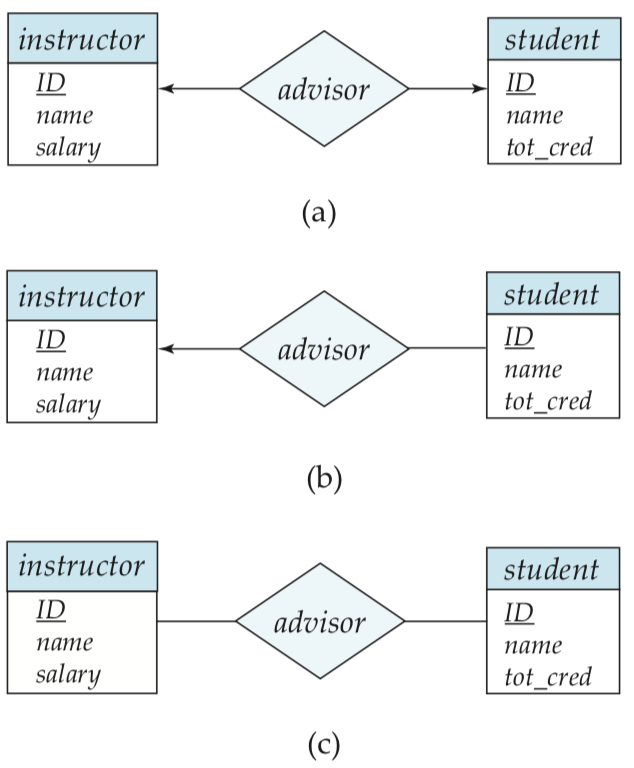
\includegraphics[width=0.5\textwidth]{images/advisor-relationship}
\end{center}


\end{frame}


\begin{frame}
\frametitle{Specific Numbers}

In the diagram below, an instructor can have zero or more students and a student can have exactly one advisor.

\begin{center}
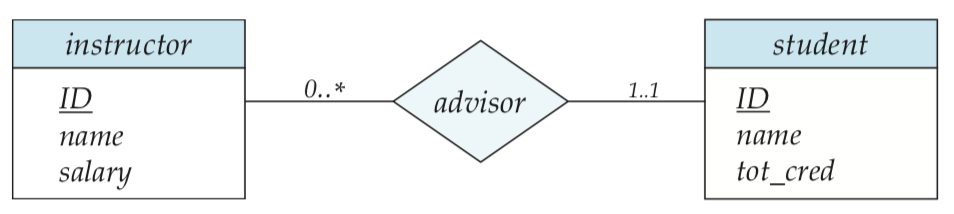
\includegraphics[width=0.9\textwidth]{images/cardinality-limits}
\end{center}

\end{frame}



\begin{frame}
\frametitle{Non-Binary Relationships}

There is no reason why a relationship must be binary.

A table may reference itself, as in the case of courses that have prerequisites.

Or a relation may involve many relations as in a ternary relationship:

\begin{center}
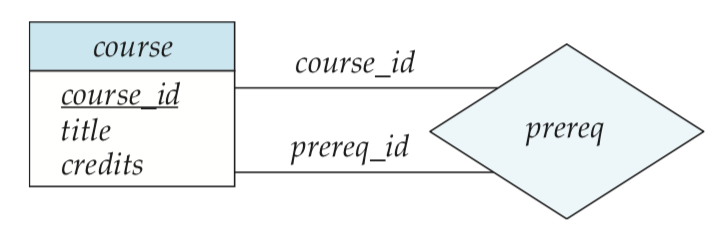
\includegraphics[width=0.5\textwidth]{images/prereq}\\
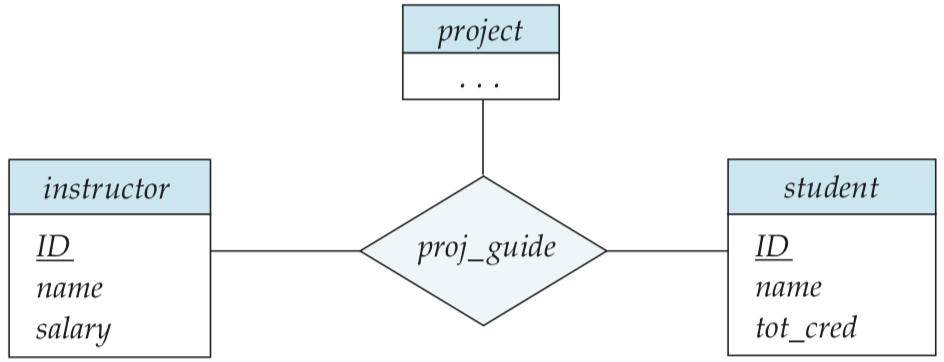
\includegraphics[width=0.5\textwidth]{images/er-ternary}
\end{center}

\end{frame}



\begin{frame}
\frametitle{Weak Entity Sets}

Weak entity sets are not entities that do not even lift. 

Instead, they are entities that are dependent on another entity, namely, one that cannot be identified uniquely based on its own attributes. 

The example that builds on this ``university'' model is a section: a section of a course, such as 001, is dependent on a course in a particular term. 

\end{frame}


\begin{frame}
\frametitle{Weak Entity Set: Section}

Suppose that a course has an id, name, and code. 

A section has a section number, year, and term. 

A particular course, ECE 356, will have one ore more sections, e.g. 001. 

But the attributes of the section on their own (001, 2018, Winter) are not enough to uniquely identify a single course. 

\end{frame}

\begin{frame}
\frametitle{Weak Entity Set: Section}

Because at least one another course, such as ECE 459, also has a section that matches (001, 2018, Winter). 

To differentiate between two sections that match on those same criteria we need a course number, but the course number isn't a part of the section entity. 

That is part of the course entity. And this is what makes the section entity a weak entity.

\end{frame}



\begin{frame}
\frametitle{Weak Entity Set}

More formally, an entity that on its own does not possess sufficient attributes to form a primary key is a weak entity. 

One that is not weak is a strong entity. 

A weak entity set is associated with another entity, called its identifying set or its owner entity set.

\end{frame}



\begin{frame}
\frametitle{If Lost, Please Return To...}

In a practical sense the weak entity will probably have some attribute added to it that identifies which strong entity the weak entity belongs to. 

That is called the \alert{discriminator}. 

That would mean some attribute added to the section entity that references a particular course. 

\end{frame}



\begin{frame}
\frametitle{If Lost, Please Return To...}


Still, that is an implementation detail that plays no role in the E-R diagram, which looks like the diagram below:

\begin{center}
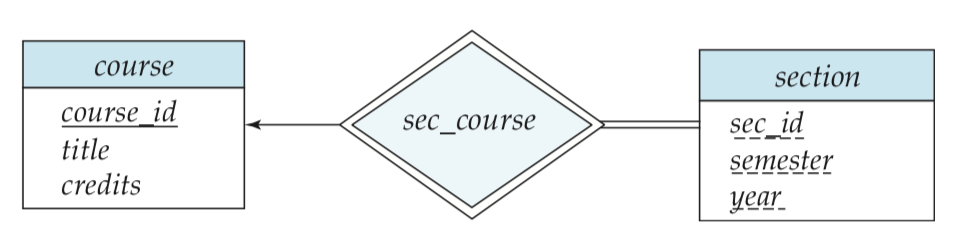
\includegraphics[width=0.7\textwidth]{images/weak-entity-set}
\end{center}


\end{frame}


\begin{frame}
\frametitle{Design Alternative: Strong Entity}

We could choose a different option, of course, and add some sort of unique identifier to the section that would promote the weak entity to a strong one. 

But that doesn't necessarily make logical sense in the context of the application. 

A section doesn't make sense on its own and giving it a unique identifier does not really correspond with reality. 

A section is logically dependent on the course, isn't it?


\end{frame}



\begin{frame}
\frametitle{Weak Entities}

Weak entity sets can exist in other configurations than just the identifying relationship. 

A weak entity can be the owner of another weak entity, or a weak entity can belong to more than one identifying set.

\end{frame}


\begin{frame}
\frametitle{When to Use Weak Entities}

When does it make sense to have a weak entity? 

You might ask yourself if a particular entity can exist independently of any other entity. 

In an e-commerce scenario, there are customers, who have orders composed of items. 

Customers can exist if they don't have any orders, and items can exist if they don't appear in any orders. 

In that case, we would expect that both customer and order both to be strong entities.

\end{frame}



\begin{frame}
\frametitle{Customer Reviews}

Continuing this analogy, what about product reviews? 

A review belongs to an item, and if it is not anonymous then it also belongs to a user. 

But a review does not make sense independent of an item, otherwise, what would it be a review of? 

In this case, review can be modelled as a weak entity and it can have one identifying set (item) or two (item and customer).

We could assign it an ID and promote it to a strong entity...

There must be at least SOME strong entities in the system.

\end{frame}



\begin{frame}
\frametitle{Specialization and Generalization}

\alert{Specialization} is the same as a subclass in object-oriented-programming.

 We have some parent class (e.g., user) that has some number of attributes like ID, name, email, et cetera. 
 
 And then there are some particular classifications: a staff member is a user, but has certain staff specific attributes like office and phone number. 
 
 A customer is a user but has different attributes like frequent flyer number, airline status, et cetera. 

\end{frame}




\begin{frame}
\frametitle{Specialization and Generalization}

The mirror image operation of this is generalization, which is analogous to extracting a superclass in object-oriented programming. 

In that case we would identify some common attributes between certain entities. 

Consolidate the common attributes in a single entity from which the other ones are derived.

\end{frame}



\begin{frame}
\frametitle{Specialization and Generalization}
Obviously, this only works if we have attribute inheritance: sub-entities receive the attributes of their super-entities. 

As you know about OOP we don't have to go into this topic.


Note: Information hiding (encapsulation) principles aren't present in the database design.


\end{frame}



\begin{frame}
\frametitle{Specialization and Generalization}

\begin{center}
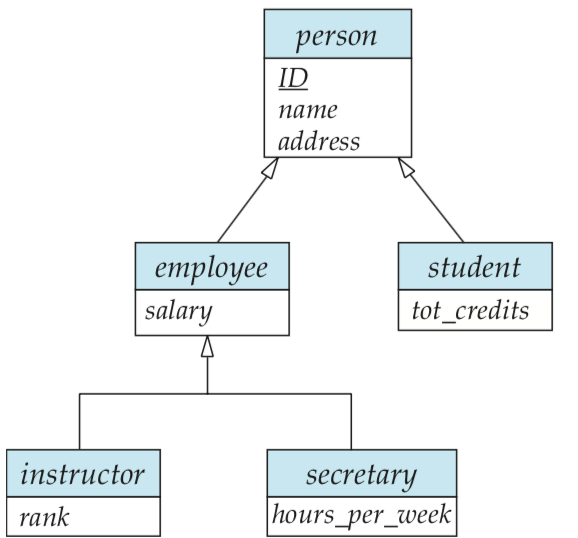
\includegraphics[width=0.5\textwidth]{images/specialization-generalization}\end{center}

\end{frame}



\begin{frame}
\frametitle{Definition of Generalization}

We have some choices about how the generalization is defined. 

The first option is to have it be \alert{condition} defined, such as having some rules that say that a person who fulfills a certain condition is included in that group. 

So a customer who has status of ``Frequent Flyer'' in the system is automatically included in that specialization. 

In other cases, an operation must be taken to specifically include a person in that subset, such as assigning an employee to a specific department

\end{frame}



\begin{frame}
\frametitle{Disjoint or Not}

We could also have rules that say sets must be disjoint (a member of some group cannot be a member of another group), or if they can be overlapping. 

In our system we could say that a staff person can also be a customer, but that is specific  to the domain we are discussing. 

We could write in some rules that say that no instance of ``user'' can exist, and everyone must be a staff member or customer (or both).

This is called \alert{total specialization}.

\end{frame}




\begin{frame}
\frametitle{Aggregation}
Aggregation allows us to treat a grouping of entities that are related as a single block. 

This can simplify the diagram and show us a relationship between relationships. 

Aggregation may not seem very useful in the context of a database schema that can be handily represented on a piece of paper.

For a large database it can be a good way to sequester parts of the design in a different area so the diagram is comprehensible.

\end{frame}



\begin{frame}
\frametitle{Aggregation Example}

\begin{center}
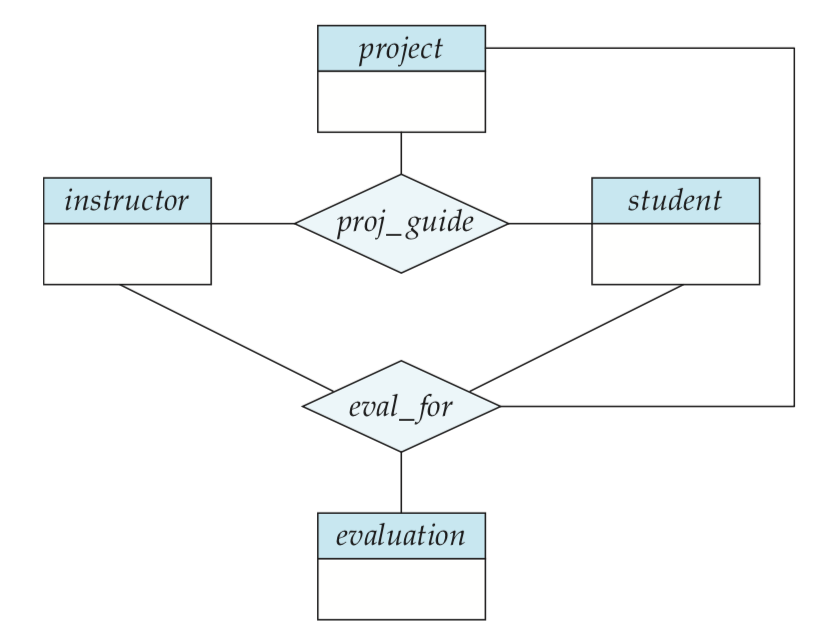
\includegraphics[width=0.45\textwidth]{images/unaggregated}
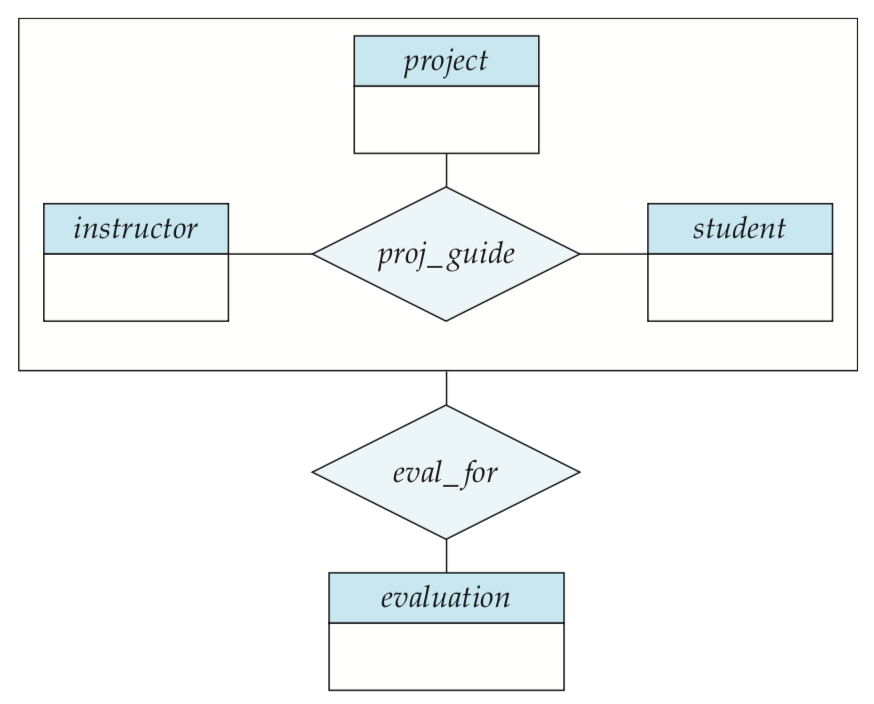
\includegraphics[width=0.42\textwidth]{images/aggregation}
\end{center}


\end{frame}



\begin{frame}
\frametitle{Aggregation Example}

It looks like the relationship \textit{eval\_for} and \textit{proj\_guide} can be combined because they seem to connect the same three things. 

But we may not want to do that if some sets of (instructor, student, project) do not have an associated evaluation. 

Now possibly the data is redundant! 

If the evaluation is a simple enough element (e.g., it is an enumeration or an integer letter grade) then it could be an attribute of the \textit{proj\_guide} relationship. 

But this option is not suitable if the evaluation relation is used in some other relationship or in some other context. 

We  also might not be able to combine it if there are multiple evaluations on a project...

\end{frame}



\begin{frame}
\frametitle{Aggregation Example}

We can consider \textit{proj\_guide} a higher level entity,  leaving a binary relationship between that aggregated entity and the evaluation relation.

The textbook contains a couple of alternative diagram notations. 

You may encounter them in the real world, but we will not invest any time discussing them as they could be confusing.

Given a good understanding of how diagrams are formed, we will next think about how to turn models into tables, and what makes up a good design.



\end{frame}



\end{document}

